% fig-jointmon: drift-monitor design space (4 panels a–d)
% Data digests: R/jointmon_panel_{a,b,c,d}.csv
% Fragments:    out/jointmon-panel-{a,b,c,d}.tex  (emitted by R/jointmon.R)
%
% Layout (matches historical make_fig_jointmon.py science; tightened chrome):
%   a|b top row (tight horizontal gap), c full-width middle, d full-width heatmap
% Chrome: gutter \panellabel; shared a/b legend above titles; titles near axes.
% Legend↔title gap uses ~26pt above axis-north (titles stay @1.015).
% Height budget: a|b taller share (~1.80in); c/d shorter; legends @26pt;
% ~0.16in between c-legend south and a/b axis-south (xlabel clearance).
\documentclass[border=2pt]{standalone}
% inspect_style.tex: Shared style definitions for all Inspect figures
% Enforces uniform fonts, colors, and panel label positioning

\usepackage[T1]{fontenc}
\usepackage{lmodern}  % Latin Modern for Type 1 fonts
\usepackage{amssymb}  % \blacksquare for shared legends
\usepackage{pgfplots}
\usepackage{pgfplotstable}
\pgfplotsset{compat=1.18}

% Color palette (Okabe-Ito colorblind-safe, print-safe)
% -- Backbones (used wherever PatchCore vs Dinomaly are distinguished)
\definecolor{cPatchcore}{HTML}{0072B2}   % blue
\definecolor{cDinomaly}{HTML}{D55E00}    % vermillion
% -- Decision classes / gates
\definecolor{cAccept}{HTML}{009E73}      % green
\definecolor{cDefer}{HTML}{E69F00}       % orange
\definecolor{cReject}{HTML}{D55E00}      % red
\definecolor{cControl}{HTML}{56B4E9}     % light blue
\definecolor{cTransfer}{HTML}{CC79A7}    % pink
% -- Benchmarks (canonical palette; used wherever MVTec/VisA/MPDD are
%    distinguished, so benchmark colouring is uniform across all figures and
%    never collides with the backbone blue/vermillion above)
\definecolor{cMVTecAD}{HTML}{0072B2}     % blue
\definecolor{cVisA}{HTML}{E69F00}        % orange
\definecolor{cMPDD}{HTML}{009E73}        % green

% Typography defaults
\newcommand{\figfont}{\fontsize{8}{9.5}\selectfont}
\newcommand{\axislabelfont}{\fontsize{9}{10}\selectfont}
\newcommand{\titlefont}{\fontsize{9}{10}\selectfont}
\newcommand{\tickfont}{\fontsize{7}{8}\selectfont}
\newcommand{\panellabelfont}{\fontsize{9}{10}\selectfont\bfseries}

% Panel label OUTSIDE the axis (axis clip would otherwise swallow it).
% Usage after \end{axis}: \panellabel{axname}{a}
% Parked in the left gutter at the top of the axis frame — NOT on the
% title baseline — so titles can stay truly centered over the plot box.
\newcommand{\panellabel}[2]{%
  \node[anchor=south east, font=\panellabelfont, inner sep=0.5pt]
    at ([xshift=-8pt, yshift=7pt] #1.north west) {\textbf{#2}};%
}

% Standard axis styles. Titles centered above the plot box only.
\pgfplotsset{
  inspect/centertitle/.style={
    title style={at={(0.5,1.10)}, anchor=south, font=\titlefont},
  },
  inspect default/.style={
    axis x line=bottom,
    axis y line=left,
    xlabel style={font=\axislabelfont},
    ylabel style={font=\axislabelfont},
    inspect/centertitle,
    x tick label style={font=\tickfont},
    y tick label style={font=\tickfont},
    legend style={font=\tickfont, draw=none, fill=none},
  }
}

\usetikzlibrary{calc}

\definecolor{cCatch}{HTML}{009E73}
\definecolor{cFalseAlarm}{HTML}{D55E00}
\definecolor{cG1}{HTML}{0072B2}
\definecolor{cG2}{HTML}{CC79A7}
\definecolor{cHeat}{HTML}{B2182B}

\begin{document}
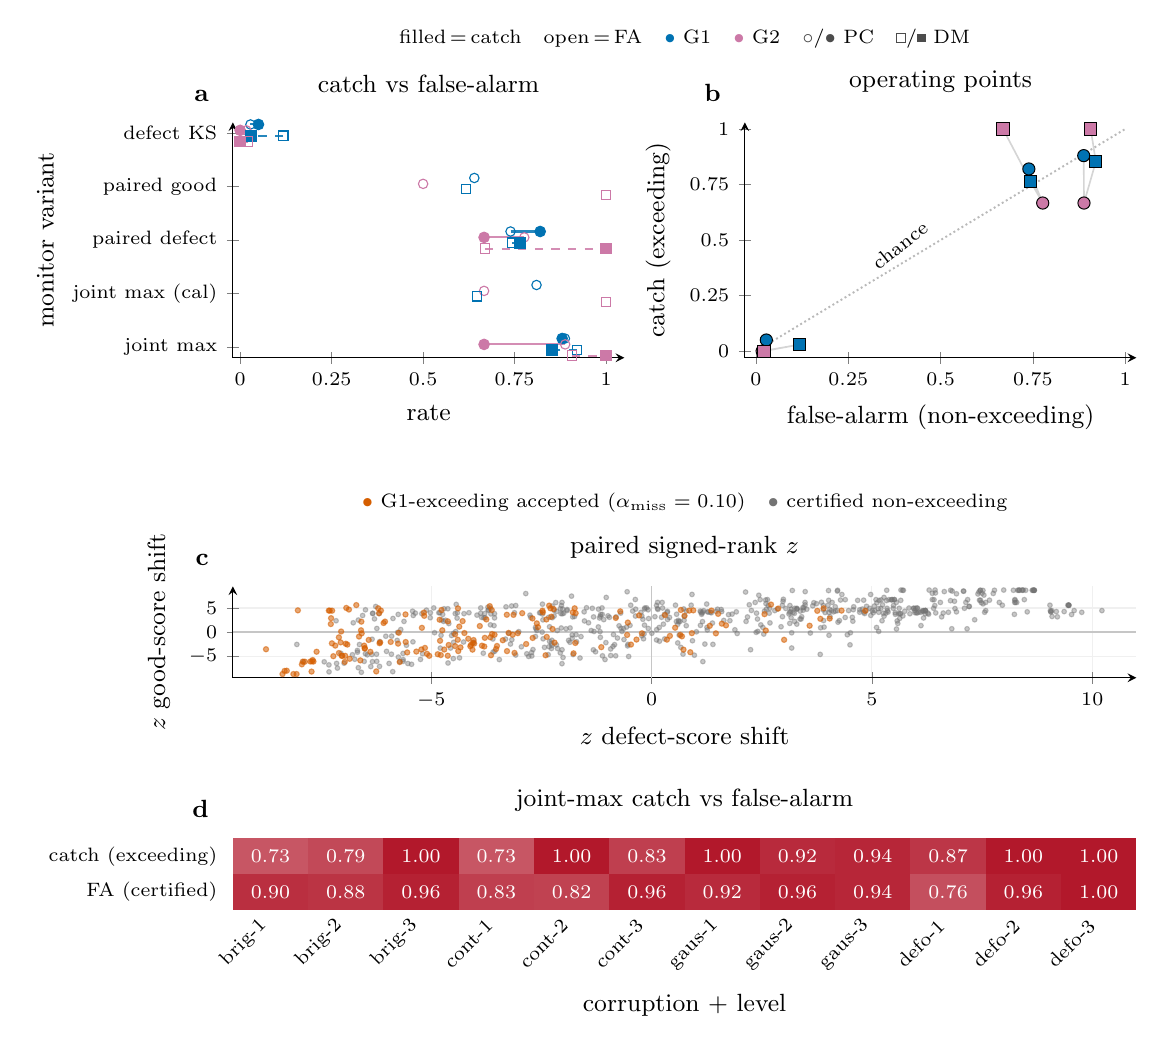
\begin{tikzpicture}[font=\figfont]

\pgfplotsset{
  jm/title near axis/.style={
    title style={at={(0.5,1.015)}, anchor=south, font=\titlefont},
  },
}

% ── Panel a: catch (filled) vs false-alarm (open) dumbbells ─────────────────
% Compact categorical band height; within-row ARM_DY from R (±0.16).
\begin{axis}[
  inspect default,
  name=ax_a,
  width=2.58in, height=1.80in, at={(0.66in,2.78in)},
  xmin=-0.02, xmax=1.05,
  ymin=-4.20, ymax=0.20,
  xlabel={rate},
  ylabel={monitor variant},
  ytick={0,-1,-2,-3,-4},
  yticklabels={defect KS, paired good, paired defect, joint max (cal), joint max},
  y tick label style={font=\tickfont},
  xtick={0,0.25,0.5,0.75,1},
  axis lines=left,
  clip=false,
  jm/title near axis,
  title={catch vs false-alarm},
]
% generated by jointmon.R — panel a dumbbells
\draw[cG1, solid, line width=0.75pt, opacity=0.85] (axis cs:0.0281124497992,0.16) -- (axis cs:0.05,0.16);
\addplot[cG1, only marks, mark=o, mark size=1.7pt, forget plot] coordinates {(0.0281124497992,0.16)};
\addplot[cG1, only marks, mark=*, mark size=1.9pt, forget plot] coordinates {(0.05,0.16)};
\draw[cG2, solid, line width=0.75pt, opacity=0.85] (axis cs:0.0167597765363,0.05) -- (axis cs:0,0.05);
\addplot[cG2, only marks, mark=o, mark size=1.7pt, forget plot] coordinates {(0.0167597765363,0.05)};
\addplot[cG2, only marks, mark=*, mark size=1.9pt, forget plot] coordinates {(0,0.05)};
\draw[cG1, dashed, line width=0.75pt, opacity=0.85] (axis cs:0.117994100295,-0.05) -- (axis cs:0.0294117647059,-0.05);
\addplot[cG1, only marks, mark=square, mark size=1.7pt, forget plot] coordinates {(0.117994100295,-0.05)};
\addplot[cG1, only marks, mark=square*, mark size=1.9pt, forget plot] coordinates {(0.0294117647059,-0.05)};
\draw[cG2, dashed, line width=0.75pt, opacity=0.85] (axis cs:0.0215827338129,-0.16) -- (axis cs:0,-0.16);
\addplot[cG2, only marks, mark=square, mark size=1.7pt, forget plot] coordinates {(0.0215827338129,-0.16)};
\addplot[cG2, only marks, mark=square*, mark size=1.9pt, forget plot] coordinates {(0,-0.16)};
\addplot[cG1, only marks, mark=o, mark size=1.7pt, forget plot] coordinates {(0.64,-0.84)};
\addplot[cG2, only marks, mark=o, mark size=1.7pt, forget plot] coordinates {(0.5,-0.95)};
\addplot[cG1, only marks, mark=square, mark size=1.7pt, forget plot] coordinates {(0.617647058824,-1.05)};
\addplot[cG2, only marks, mark=square, mark size=1.7pt, forget plot] coordinates {(1,-1.16)};
\draw[cG1, solid, line width=0.75pt, opacity=0.85] (axis cs:0.738955823293,-1.84) -- (axis cs:0.82,-1.84);
\addplot[cG1, only marks, mark=o, mark size=1.7pt, forget plot] coordinates {(0.738955823293,-1.84)};
\addplot[cG1, only marks, mark=*, mark size=1.9pt, forget plot] coordinates {(0.82,-1.84)};
\draw[cG2, solid, line width=0.75pt, opacity=0.85] (axis cs:0.776536312849,-1.95) -- (axis cs:0.666666666667,-1.95);
\addplot[cG2, only marks, mark=o, mark size=1.7pt, forget plot] coordinates {(0.776536312849,-1.95)};
\addplot[cG2, only marks, mark=*, mark size=1.9pt, forget plot] coordinates {(0.666666666667,-1.95)};
\draw[cG1, dashed, line width=0.75pt, opacity=0.85] (axis cs:0.743362831858,-2.05) -- (axis cs:0.764705882353,-2.05);
\addplot[cG1, only marks, mark=square, mark size=1.7pt, forget plot] coordinates {(0.743362831858,-2.05)};
\addplot[cG1, only marks, mark=square*, mark size=1.9pt, forget plot] coordinates {(0.764705882353,-2.05)};
\draw[cG2, dashed, line width=0.75pt, opacity=0.85] (axis cs:0.669064748201,-2.16) -- (axis cs:1,-2.16);
\addplot[cG2, only marks, mark=square, mark size=1.7pt, forget plot] coordinates {(0.669064748201,-2.16)};
\addplot[cG2, only marks, mark=square*, mark size=1.9pt, forget plot] coordinates {(1,-2.16)};
\addplot[cG1, only marks, mark=o, mark size=1.7pt, forget plot] coordinates {(0.81,-2.84)};
\addplot[cG2, only marks, mark=o, mark size=1.7pt, forget plot] coordinates {(0.666666666667,-2.95)};
\addplot[cG1, only marks, mark=square, mark size=1.7pt, forget plot] coordinates {(0.647058823529,-3.05)};
\addplot[cG2, only marks, mark=square, mark size=1.7pt, forget plot] coordinates {(1,-3.16)};
\draw[cG1, solid, line width=0.75pt, opacity=0.85] (axis cs:0.887550200803,-3.84) -- (axis cs:0.88,-3.84);
\addplot[cG1, only marks, mark=o, mark size=1.7pt, forget plot] coordinates {(0.887550200803,-3.84)};
\addplot[cG1, only marks, mark=*, mark size=1.9pt, forget plot] coordinates {(0.88,-3.84)};
\draw[cG2, solid, line width=0.75pt, opacity=0.85] (axis cs:0.888268156425,-3.95) -- (axis cs:0.666666666667,-3.95);
\addplot[cG2, only marks, mark=o, mark size=1.7pt, forget plot] coordinates {(0.888268156425,-3.95)};
\addplot[cG2, only marks, mark=*, mark size=1.9pt, forget plot] coordinates {(0.666666666667,-3.95)};
\draw[cG1, dashed, line width=0.75pt, opacity=0.85] (axis cs:0.920353982301,-4.05) -- (axis cs:0.852941176471,-4.05);
\addplot[cG1, only marks, mark=square, mark size=1.7pt, forget plot] coordinates {(0.920353982301,-4.05)};
\addplot[cG1, only marks, mark=square*, mark size=1.9pt, forget plot] coordinates {(0.852941176471,-4.05)};
\draw[cG2, dashed, line width=0.75pt, opacity=0.85] (axis cs:0.906474820144,-4.16) -- (axis cs:1,-4.16);
\addplot[cG2, only marks, mark=square, mark size=1.7pt, forget plot] coordinates {(0.906474820144,-4.16)};
\addplot[cG2, only marks, mark=square*, mark size=1.9pt, forget plot] coordinates {(1,-4.16)};

\end{axis}
\panellabel{ax_a}{a}

% ── Panel b: operating points vs chance diagonal ────────────────────────────
\begin{axis}[
  inspect default,
  name=ax_b,
  width=2.58in, height=1.80in, at={(3.22in,2.78in)},
  xmin=-0.03, xmax=1.03,
  ymin=-0.03, ymax=1.03,
  xlabel={false-alarm (non-exceeding)},
  ylabel={catch (exceeding)},
  xtick={0,0.25,0.5,0.75,1},
  ytick={0,0.25,0.5,0.75,1},
  axis lines=left,
  clip=false,
  jm/title near axis,
  title={operating points},
]
\addplot[gray!55, densely dotted, line width=0.7pt, forget plot, mark=none]
  coordinates {(0,0) (1,1)};
% "chance" sits in the empty mid-diagonal band (clear of the ~0.67–0.92 cluster
% and its grey connectors). Slightly above y=x so the dotted line does not
% run through the letters; keep annotation chrome black / not bold.
\node[font=\tickfont, text=black, rotate=38, anchor=west]
  at (axis cs:0.30,0.36) {chance};
% generated by jointmon.R — panel b operating points
\addplot[gray!50, line width=0.6pt, solid, opacity=0.65, forget plot, mark=none] coordinates {(0.0281124497992,0.0500000000000) (0.0167597765363,0.0000000000000) (0.1179941002950,0.0294117647059) (0.0215827338129,0.0000000000000)};
\addplot[gray!50, line width=0.6pt, solid, opacity=0.65, forget plot, mark=none] coordinates {(0.738955823293,0.820000000000) (0.776536312849,0.666666666667) (0.743362831858,0.764705882353) (0.669064748201,1.000000000000)};
\addplot[gray!50, line width=0.6pt, solid, opacity=0.65, forget plot, mark=none] coordinates {(0.887550200803,0.880000000000) (0.888268156425,0.666666666667) (0.920353982301,0.852941176471) (0.906474820144,1.000000000000)};
\addplot[cG1, only marks, mark=*, mark size=2.2pt, mark options={draw=black, line width=0.35pt}, forget plot] coordinates {
(0.0281124497992,0.05)
(0.7389558232932,0.82)
(0.8875502008032,0.88)
};
\addplot[cG2, only marks, mark=*, mark size=2.2pt, mark options={draw=black, line width=0.35pt}, forget plot] coordinates {
(0.0167597765363,0.000000000000)
(0.7765363128492,0.666666666667)
(0.8882681564246,0.666666666667)
};
\addplot[cG1, only marks, mark=square*, mark size=2.2pt, mark options={draw=black, line width=0.35pt}, forget plot] coordinates {
(0.117994100295,0.0294117647059)
(0.743362831858,0.7647058823529)
(0.920353982301,0.8529411764706)
};
\addplot[cG2, only marks, mark=square*, mark size=2.2pt, mark options={draw=black, line width=0.35pt}, forget plot] coordinates {
(0.0215827338129,0)
(0.6690647482014,1)
(0.9064748201439,1)
};

\end{axis}
\panellabel{ax_b}{b}

% Shared a/b legend — above the title row (breathing room vs titles @1.015).
% South anchor @26pt clears title tops (~10pt) without dropping onto the spine.
\node[anchor=south, font=\tickfont, text=black, inner sep=0.5pt]
  at ($(ax_a.north)!0.5!(ax_b.north)+(0,26pt)$) {%
  filled\,=\,catch\quad open\,=\,FA\quad
  \textcolor{cG1}{$\bullet$}~G1\quad
  \textcolor{cG2}{$\bullet$}~G2\quad
  \textcolor{black!70}{$\circ$}/\textcolor{black!70}{$\bullet$}~PC\quad
  \textcolor{black!70}{\tikz[baseline=-0.15ex]\draw[line width=0.45pt] (0,0) rectangle (1.05ex,1.05ex);}/\textcolor{black!70}{\rule[0.15ex]{1.05ex}{1.05ex}}~DM%
};

% ── Panel c: per-cell signed-rank $z$ cloud ─────────────────────────────────
% Axis limits padded from frozen z ranges (~[-8.7,10.2] × [-8.7,8.7]).
\begin{axis}[
  inspect default,
  name=ax_c,
  width=5.14in, height=1.08in, at={(0.66in,1.18in)},
  xmin=-9.5, xmax=11.0,
  ymin=-9.5, ymax=9.5,
  xlabel={$z$ defect-score shift},
  ylabel={$z$ good-score shift},
  xtick={-5,0,5,10},
  ytick={-5,0,5},
  axis lines=left,
  xmajorgrids, ymajorgrids, grid style={gray!12},
  clip=false,
  jm/title near axis,
  title={paired signed-rank $z$},
]
\draw[gray!45, line width=0.45pt] (axis cs:0,-9.5) -- (axis cs:0,9.5);
\draw[gray!45, line width=0.45pt] (axis cs:-9.5,0) -- (axis cs:11.0,0);
% generated by jointmon.R — panel c scatter
\addplot[black!55, only marks, mark=*, mark size=0.85pt, opacity=0.40, forget plot] coordinates {
(6.21091719733054,3.8079323040274)
(-2.26271320086675,-2.8066011465212)
(-3.31217445245405,-1.4599177552139)
(-0.63739574701450,0.7286855487700)
(5.97956580677345,4.0145085713905)
(6.81267059596469,0.6855061627637)
(5.55801026622801,0.6330801796250)
(9.76188513265826,4.1017733272718)
(-2.95340153808474,-3.0594117081557)
(5.44244918805467,6.7285051434866)
(4.23090415099791,2.0523512732931)
(3.11835019615915,3.7584868998340)
(1.94318183445712,-0.2986613571786)
(3.16682106730378,2.9691904543197)
(6.01033544214278,4.0145085713905)
(0.36230545457580,2.6076116779638)
(6.73586674648826,4.1069047550031)
(7.33183603261046,2.5524967144942)
(0.22643927924945,3.0643326984944)
(-1.03581195394767,-2.1965007135477)
(1.18193546761362,4.4390466099808)
(3.24606888154664,2.2133200006102)
(1.14481504720633,3.9267773580355)
(0.61016341967910,2.4266235270763)
(-1.08396090544653,2.5820730547995)
(1.25758280405507,0.9732785034760)
(0.78737121690027,1.3207425571457)
(4.97442438470861,3.4583861718905)
(6.42710938238012,5.5109318967277)
(6.10895070696407,4.1069047550031)
(9.20846300287976,3.1620481687018)
(-2.32689460497759,-3.0594117081557)
(5.16334922969289,6.5665498774508)
(4.56782148002072,2.2535621824395)
(2.68681406267761,1.9039661520137)
(4.44234621941225,-0.5613202293042)
(8.23316225634335,3.6802093412685)
(-5.90230443680437,-4.5998275266107)
(6.03084853238900,3.9797509214217)
(-0.18206031560747,-1.3978949201456)
(4.02679684188970,-0.6655458298622)
(5.15404435645896,0.1396888749226)
(4.39378248455386,3.0285970402029)
(-1.60080029246458,-0.9413574486633)
(5.44244918805467,6.6916971284785)
(-2.61951754923245,0.6438749092684)
(0.74343172272850,3.2723144650296)
(5.57343302751655,2.3146255181343)
(7.20354051420645,5.2918948514406)
(6.17282219175048,2.9198355104279)
(2.56294548807419,4.3493418692210)
(-6.01313960144110,-4.0145085713905)
(3.44190181847006,4.5431584904730)
(-0.54335816478461,-2.8732100459903)
(9.36245872594856,4.2541611908236)
(2.40399905102022,2.7069761155796)
(3.29576530801531,1.6473755351607)
(1.10942408923242,1.3913429673074)
(0.59392402667561,1.6096872731711)
(3.93897805593650,4.0608615209665)
(6.11343244125859,1.3382579422794)
(4.72422730140159,4.6225989500098)
(5.70263908844946,3.3541132219842)
(3.43359367154446,5.0808103828367)
(6.44876422942482,3.9770421540543)
(9.53089154805506,3.6446097366161)
(-2.15825497013885,-2.6671794378793)
(-0.42781713244910,4.3580689769629)
(-1.30409486248766,0.1207265454878)
(5.31608515531436,3.9199303129694)
(0.78821021642933,4.3628130925923)
(-5.63876294905608,-4.4404275628173)
(-1.78838482121634,3.1455673221717)
(0.17490608151935,0.9543321089455)
(5.63162629624428,2.8407443957531)
(6.58271882525649,3.1620481687018)
(1.38127960342165,1.8671881457298)
(2.47967104126866,1.4904826270502)
(5.38662919638232,6.7358667464883)
(5.64540416934821,3.8230072737813)
(5.48368538789262,4.9365201072447)
(0.89894658377176,5.5783617270856)
(1.92325610520010,4.1972635462401)
(-3.23568546922131,-0.2504856573897)
(-4.76172116887303,2.5199296227343)
(1.46606464673387,4.3012151389094)
(3.90383857640796,2.3862252924326)
(4.08218385725032,4.4573450088928)
(0.13549108983206,4.8868512713599)
(-2.27184733698826,-2.3533936216582)
(5.09357424010245,6.7358667464883)
(5.60789317818975,3.8230072737813)
(-4.45406202141956,3.8440757772352)
(-1.52951796995410,4.1972635462401)
(-3.64411269961584,3.7712050216092)
(5.49055583384644,5.5109318967277)
(6.40014712940353,4.9365201072447)
(-1.91766410572440,4.4573450088928)
(-1.85190622069432,-2.1180542594924)
(4.01903940040960,6.5959962894574)
(-1.11796341841905,3.6620385464642)
(-6.16675583297192,-1.9786314913084)
(0.92854321417858,-1.8000959077688)
(-6.34022925643840,-1.4903327084476)
(-6.24016959288826,-4.5998275266107)
(3.91539872100619,1.0253506740781)
(-6.67250601447101,-4.1802434631276)
(6.61808109846223,3.9445765038172)
(9.08815384423226,3.2382421004777)
(-5.35924698518410,3.9398563266357)
(-0.56796183424706,1.0198039027186)
(4.02438150015681,4.0930512689043)
(5.64540416934821,3.8230072737813)
(6.16405216945991,4.3194550938391)
(3.24206234933969,3.8825976433221)
(1.11753491579222,4.1382850008706)
(-3.57369739172194,1.3382579422794)
(-5.19619115357319,-4.4859704096154)
(5.86251592280386,3.8059626715780)
(4.57772254433886,4.6372475716367)
(6.28680896338904,3.7173169521569)
(9.18440117115026,4.2541611908236)
(-5.42211444773757,4.3329485678419)
(-0.17038855027412,-0.3922322702764)
(5.05404307316990,5.4034166031939)
(0.56891669923664,3.7022807282935)
(-0.36427666846513,3.3226075986122)
(-4.77606651339233,-0.6777741743906)
(3.89992360274956,5.5109318967277)
(9.07852911154046,4.4573450088928)
(3.65779367483868,5.4489898790034)
(-2.48202091197609,0.0000000000000)
(5.33080920470996,6.5371034654443)
(-3.56211096698017,2.9376792735372)
(-4.49104429004526,-2.1279621698977)
(2.24677809912182,-3.6660017734560)
(-1.52220606074636,2.3115364457554)
(-4.55976982394994,-3.3246278162632)
(-1.31493193866228,3.1455673221717)
(-6.62759681930773,-2.5941703806547)
(-1.11365430909678,-4.9365201072447)
(-8.04824636429901,-2.5722342235010)
(-6.02961877078546,-0.8665897135684)
(0.62733435032427,-0.6275716324422)
(-0.92744951432734,-3.5114846317758)
(-5.89664400430283,-0.8450858184148)
(-4.44312156134051,0.1119980089420)
(5.84084427847960,4.9822009318245)
(0.61825449736371,2.1290467263537)
(-7.15775442530320,2.3454566101035)
(-2.51465836003994,4.0145085713905)
(-5.86681307846004,2.8226724349093)
(-0.92674729218543,-4.8804232878441)
(3.20954931961259,4.0509773727545)
(-6.65339378188672,2.4944840706496)
(-6.55587248006999,3.4395571105549)
(3.13667175162135,1.8042684432713)
(0.73927135200005,2.4440521965400)
(-6.28680896338904,2.7364683643908)
(-2.75897995257353,3.5092709468488)
(7.46459898789693,6.6235787057900)
(5.03219858612178,4.0147738268383)
(-3.11054896668448,4.0145085713905)
(-3.17480907238361,5.4168428155640)
(-0.07787792371306,4.6186381306418)
(5.15540891975196,4.1069047550031)
(9.58954476097138,4.4573450088928)
(-0.47202235678591,5.5785734670891)
(4.55588716710904,3.0594117081557)
(2.98396800261839,6.3825098024102)
(-6.18374652136627,3.8230072737813)
(-1.80052537847851,-0.5973227143572)
(1.16427495951027,-6.1358107823946)
(0.56383600859820,2.1898766328209)
(-1.27035310034675,-4.0988562118313)
(-4.73931662484621,3.6669320717030)
(-6.67441428028297,-3.8173284357821)
(-0.81382430280149,-4.9365201072447)
(-1.84831226224593,0.8487725019613)
(-5.41416951755440,-2.0279986080415)
(-1.88200305097281,-1.7258219892160)
(-2.06995978560015,-4.3359841679580)
(-5.77149675327518,-1.7304138186589)
(-7.04586180887725,-4.4316487326401)
(2.66998059926471,3.9199303129694)
(3.89779008183872,4.6105682282852)
(8.52405161524202,4.1972635462401)
(-4.40561788512527,4.0145085713905)
(-6.76804920223346,1.9221055152001)
(-1.77951055684345,-4.6747349500423)
(9.04002367574804,5.5785734670891)
(-4.94143313463779,5.0119260753801)
(-1.36779456710046,0.3137858162211)
(0.26882594618184,1.6342758663611)
(-5.02061324710928,2.9779214553665)
(6.27103135622173,3.9199303129694)
(7.44123561078301,6.6235787057900)
(9.05916675476954,4.1972635462401)
(-4.82671391382074,4.0145085713905)
(-4.70808091932280,4.8388670312731)
(1.13606744311145,3.6848513019197)
(2.79587864744707,4.4573450088928)
(9.46696524564990,5.5785734670891)
(-3.87554638447675,5.0119260753801)
(-2.25223315936090,2.9809652541004)
(4.67757146356397,6.5812730834541)
(-3.56301585278723,3.8230072737813)
(6.03287000948278,4.9365201072447)
(-6.32580018902716,3.9199303129694)
(5.65393726156825,6.5848669658380)
(-0.24034832538100,4.1060186865392)
(-6.32835824256497,3.8407203215467)
(-6.25890931412770,5.3093124370913)
(-2.01703822416829,4.7869285888433)
(9.44575075770447,5.5785734670891)
(-2.06933661955951,4.8689834422141)
(-3.77429027162307,2.9809652541004)
(4.39530422007304,6.7285051434866)
(-5.69051912025729,0.5231483637806)
(-1.34446817354188,4.9365201072447)
(-3.87489492098417,3.9199303129694)
(7.66708158955089,6.6235787057900)
(6.91870619665947,4.1972635462401)
(-5.40667189084777,3.4384849332585)
(-5.01739890794699,4.0145085713905)
(-3.08117415043313,5.5109318967277)
(1.33531029991346,4.1069047550031)
(7.58293329151176,4.4573450088928)
(9.46696524564990,5.5785734670891)
(-0.15163242470910,5.0119260753801)
(-2.33450651678048,3.0594117081557)
(5.47060800480039,6.7358667464883)
(-5.61690309024103,2.2133200006102)
(2.68098091410422,4.9365201072447)
(2.38245120601157,3.9199303129694)
(8.24337822502754,6.6235787057900)
(9.06219000414540,4.1972635462401)
(-5.10800594455047,4.5542846798126)
(-4.14342601820167,4.0145085713905)
(3.13969597665218,5.5109318967277)
(7.55781798157617,4.1069047550031)
(10.21931205292486,4.4573450088928)
(9.46696524564990,5.5785734670891)
(-0.11149442993316,5.0119260753801)
(-0.95642778000258,3.0594117081557)
(5.51093189672766,6.7358667464883)
(-5.21201492515157,3.8230072737813)
(5.98778922259873,4.9365201072447)
(-2.46459747624435,2.5386215360183)
(-2.72183343377149,-4.2621625687170)
(0.29476681414651,3.6802093412685)
(-3.70877644271926,4.5315132564135)
(-6.23301574550185,0.7472894743281)
(-4.49155016231230,-0.2553846488727)
(-3.55512721750125,-3.9828741774360)
(-5.76106191470574,-0.0712709734471)
(-1.71255444377339,-0.5449687889451)
(-3.01326171549199,0.0784464540553)
(1.74736865018194,3.6145470737986)
(-4.71878752404259,2.2133200006102)
(-3.78589556767535,3.8452649736748)
(-3.30202396543380,5.2376984155078)
(1.28941585880501,4.1668485930064)
(-3.69650249972074,4.5998275266107)
(-5.74835805209762,3.6669320717030)
(-3.71320987359890,5.1748994640004)
(-4.62205477237019,4.8430254082438)
(2.96737650136757,5.5396983906634)
(0.24974752305029,4.9940582462343)
(-4.41190879162479,2.9025188000451)
(4.28777384160030,6.6548891134704)
(-4.67461790603283,2.4547730915859)
(-1.99221629329751,3.9199303129694)
(4.81285568546719,6.6235787057900)
(4.12824702273913,4.1972635462401)
(-6.49087018905031,4.6225989500098)
(-4.80287828955496,4.0145085713905)
(-2.04533782635590,5.5109318967277)
(-3.65636851832823,4.9365201072447)
(3.13232760453157,4.1069047550031)
(9.05033224302428,4.4573450088928)
(9.46696524564990,5.5785734670891)
(-1.12386385372628,5.0119260753801)
(-3.85656362904264,3.0594117081557)
(5.51093189672766,6.7358667464883)
(-4.25500653494012,3.8230072737813)
(4.95093112426565,4.9365201072447)
(3.83692585744758,0.8939644593377)
(-0.83910760167422,-2.6112118814466)
(-3.81751551564929,-4.3874151575507)
(4.16767492807186,5.2568964607035)
(0.07627840804155,3.1907654548668)
(6.87376327187094,6.3975519075489)
(-6.23517334991367,-6.0926646045680)
(0.36018350353295,4.3101889281549)
(6.02406786955529,5.0165159468218)
(-3.20087782257451,-2.4953725373528)
(-7.89983361496396,-6.1539651549804)
(-2.78802966892759,-5.0713910475329)
(-2.74224109393002,3.0394791617481)
(-7.31780154388848,-8.2691712488734)
(5.27563601183225,3.3012519639430)
(4.58713443959077,5.2488229401597)
(-5.56119505439190,-2.7463577828893)
(-6.52031708459956,-6.0863922042590)
(5.23003320656378,2.3449375433396)
(4.51201274264190,-0.1535727502350)
(-2.25441702904118,5.4016083293057)
(-2.03049755221508,-3.6721309329717)
(4.87782407450939,5.3406092572151)
(-1.47554363497890,5.0534913860898)
(5.25675985063164,3.9162519968677)
(-2.42897182988834,-3.1807553232408)
(-6.33306695293927,-6.1443118763059)
(5.55470236771917,6.1605085924726)
(0.64489926798763,2.2005278999081)
(-5.95497210656512,-6.5190639034778)
(7.54116300830755,7.6746909433688)
(-5.44512708282160,-6.6956639371302)
(3.15530660735277,4.2619225347825)
(3.48483419733512,5.6388527435145)
(-2.71630911690430,-4.9666118780195)
(3.52273953128441,4.7466213745281)
(-0.19647468737975,2.6543867792642)
(5.20905122735250,6.6737885214401)
(-5.63898789924591,-6.0863922042590)
(-3.08251689033107,-4.7749699904267)
(-4.53731551714703,-0.7254865420010)
(-3.45362987843436,-5.7213725397611)
(-0.86333169460343,-0.5166145967176)
(-5.24277934936399,-5.6809544999309)
(-5.71260392926217,-6.1443118763059)
(2.14518500571220,2.2165074055747)
(6.91822046267739,7.9494070384180)
(-7.12734401382777,-7.4886715093748)
(7.52120003484649,5.8623053089824)
(-0.70025793006723,3.9433643385247)
(3.82724189957629,-4.6384004030872)
(0.17953893158307,-1.8968692595351)
(4.81836732006063,4.1115613585642)
(6.44205827914530,8.1281999302856)
(-6.45016168472299,-4.7345733096460)
(2.54616323466863,-0.4217607691236)
(-0.73684599088766,1.2983659817174)
(-6.34665153454011,-4.6577069604361)
(-0.07362327122281,0.7481290972721)
(3.40715916244643,3.1838888051795)
(-2.47437317250308,3.7408974298438)
(-1.16390712814883,3.3007918498622)
(1.89089134291906,0.4710505035741)
(-3.59439718446517,-4.1460831906888)
(5.24026743092796,5.6502335062971)
(-0.67263687091183,0.1444096434315)
(-6.37026998451083,-7.1723456237630)
(7.50030179995429,8.0608815271446)
(-0.77338115767885,-1.2404463096706)
(-4.35684507207899,-5.3527430249986)
(4.72268220406947,4.1225514874841)
(7.40559920882805,7.9145792012008)
(-3.80463251111483,2.9397677412835)
(6.36980836884738,8.0473309803454)
(-7.14646791643951,-6.5161191920414)
(-6.73413570678212,-5.6519946639075)
(2.13386310289256,8.3138694718403)
(0.14388861576724,4.7059733538085)
(0.35758578373507,4.0916065638916)
(-1.62288932618223,-5.3886933971906)
(-5.74544081366632,-5.1982905662070)
(-4.79302483198734,-3.3352077820325)
(-0.62577512153637,-1.5590045059284)
(-2.04924160678942,0.8423895866836)
(-2.03204998257139,-6.5672004512883)
(-1.05556572698717,-5.7076192403866)
(-5.63541441867091,-5.7166369308916)
(-6.78725324127906,-4.7105088310546)
(-3.96095021983459,3.5186200768476)
(2.43433398927334,7.6468344521807)
(4.83428473011062,3.8427567668490)
(1.21029034494946,-2.4953725373528)
(-4.03315504155032,-2.1285479477226)
(4.00221011795787,5.5651151558372)
(3.85436214968279,6.1855463936479)
(7.75342252233246,8.0216118601338)
(2.26585607193663,4.4904522457500)
(4.97181772385488,7.8049973949866)
(0.91803273324291,7.8169716847599)
(-1.81543551742419,7.4612698312822)
(3.68244590750247,6.0960454829335)
(8.41701921714850,8.6817702301062)
(8.45827911527178,6.7358667464883)
(7.95972201294885,5.5747684345117)
(0.54325532528981,5.5844217131861)
(8.25541794949900,6.1539651549804)
(8.48922403886424,8.6783319052626)
(8.68177023010620,8.6817702301062)
(7.46116491062592,8.6714552555754)
(8.32762277121474,8.6817702301062)
(8.43421084136653,8.7248583203029)
(6.29901111348695,8.7214706836032)
(8.24166465012457,6.1539651549804)
(1.77761394414452,2.3586908427140)
(-4.61767026496341,-6.4266794204199)
(-2.34493754333957,-4.6963200751341)
(-2.00798319232503,-5.2755167956028)
(-4.49732889543719,-5.5071954837903)
(-2.26241774709302,-1.7054091224288)
(1.39252156166060,-2.5581136836432)
(-6.58439207550628,-8.3585676948072)
(-5.87265883287976,-8.2244730259065)
(-5.52882634851911,-6.5364450122402)
(-6.97636110767741,-6.4686922782444)
(-4.60047864074538,1.7617233580924)
(2.64751012957694,5.5219496988319)
(0.00687664968721,-0.2502945020553)
(3.60336443609952,-0.1978922128268)
(-1.32031673994486,-3.6923790929882)
(-2.63375683020251,-0.9218881134127)
(1.10370227479766,4.3597959016929)
(6.78381491643546,6.5190639034778)
(-1.70197079758517,-2.0079831923250)
(-0.69454161840850,0.7804997394987)
(-2.03204998257139,6.1536420651642)
(-4.43200072340867,5.7471256611897)
(0.11346471983901,5.5361553198137)
(3.19420377971036,8.6370720071393)
(6.40903750848236,6.7211435404850)
(7.21016719704265,5.3430897463242)
(4.09848321357885,6.1539651549804)
(1.25155024307273,5.8161004013736)
(6.64284359784759,8.4101425674613)
(8.34825272027637,8.6783319052626)
(7.51961643296723,8.6439486568265)
(6.78725324127906,8.6817702301062)
(5.65948269257616,8.7248583203029)
(5.71449589007386,8.6706561331063)
(7.48179485968756,6.1153520402825)
(-2.85380962019332,7.9941052613849)
(2.58905860723563,6.6696123194736)
(-1.74666902055206,3.2386749952877)
(-2.17302130115925,6.1250053189570)
(-1.20685202010585,1.0666872935299)
(7.08294917782921,8.4857857140206)
(7.07607252814200,8.5132923127695)
(2.63031850535891,6.7391166934686)
(1.59194440258977,4.2566461563847)
(5.53226467336272,3.6874425477188)
(-2.05611825647664,3.8364985625095)
(0.72892486684456,4.8025061405533)
(4.01596341733229,8.6164420580777)
(6.37121593520269,6.7358667464883)
(3.74089742984378,5.8933266307695)
(0.24068273905245,6.1539651549804)
(2.59593525692284,5.9029799094439)
(8.66114028104456,8.6817702301062)
(8.63707200713931,8.6817702301062)
(4.22226290794868,8.6748935804190)
(4.31853600356966,7.8015590701430)
(6.82163648971513,8.5114372082163)
(3.48646139141690,8.3962575604236)
(5.11278904244274,6.0670856469101)
(8.30699282215310,8.6817702301062)
(8.24510297496818,6.7358667464883)
(7.89095551607672,6.1539651549804)
(2.35181419302679,6.1539651549804)
(6.55344715191383,6.1539651549804)
(8.68177023010620,8.6817702301062)
(8.68177023010620,8.6817702301062)
(5.33628015727716,8.6817702301062)
(7.78092912108132,8.6817702301062)
(8.40670424261768,8.7248583203029)
(7.99066693654131,8.7248583203029)
(8.28636287309146,6.1539651549804)
(2.99134261393758,6.8113265479382)
(-0.48824212779211,1.3913429673074)
(-0.51918705138457,-5.0727979434387)
(0.11346471983901,-1.6458840139987)
(-1.16903044682618,0.0917061474076)
(3.45551646782445,5.0680908194759)
(-2.31399261974712,1.0968256251104)
(-6.17179309427351,-7.1345240504833)
(-7.42678166218986,-6.1821080688043)
(-7.32019359203806,-6.8210064950223)
(-6.65315857237841,-7.4070676440856)
(-4.92368117604439,-0.1303192621055)
(4.21538625826146,8.5132923127695)
(2.46527891286580,6.7285051434866)
(1.58162942805895,4.6866667964596)
(-2.47559388739662,5.7967938440247)
(2.21771952412614,5.6616479425820)
(7.43021998703346,8.3448143954328)
(5.27439031009224,7.1929755728246)
(-0.36790075826589,6.7631849673738)
(-2.15239135209762,4.2910294048208)
(-0.55357029982063,8.3725441035250)
(-1.02805912823832,7.1902588952992)
(-1.17934542135700,2.9201167990299)
(8.21071972653212,8.6817702301062)
(7.17234562376298,6.7358667464883)
(7.13108572563970,6.1539651549804)
(0.13753299374426,6.1539651549804)
(7.58150628015214,6.1539651549804)
(8.68177023010620,8.6817702301062)
(8.65426363135735,8.6817702301062)
(7.45772658578231,8.6817702301062)
(5.69730426585583,8.6817702301062)
(8.34481439543277,8.7248583203029)
(6.43310578238760,8.7248583203029)
(3.48302306657330,6.1539651549804)
(4.17119275619783,4.3557530998582)
(3.39266044978513,2.7047366251686)
(-2.83036905914918,-4.5166998129804)
(5.36697645345311,4.1511646356375)
(1.26940614569400,4.2033652363064)
(1.15576822287770,2.1699598019413)
(-2.69059774758626,-3.6434277438501)
(-2.63372586054161,0.9524241471993)
(-3.65581958976245,1.4959151840135)
(4.47114369596936,4.4573450088928)
(-0.87357069726827,-2.9790998766466)
(3.36913625973938,2.7048845780461)
(-0.98763165456503,3.3658091640304)
(6.20523506652352,4.4573450088928)
(1.63951533697750,2.4167798742001)
(2.41105512446041,0.1366285403944)
(0.29797060649478,-1.4211194248129)
(6.16774119905208,4.4573450088928)
(0.66391372992388,-3.1712998686884)
(2.17693819568542,3.1414218864284)
(5.35224958154823,4.4573450088928)
(0.59402807414242,-2.2583499064902)
(5.00543130743740,4.4573450088928)
(4.04197345452869,4.6998655425933)
(3.17979733805649,-3.3154498627197)
(7.15978823609211,0.6730463973542)
(2.37324824231728,-0.0560968194005)
(1.82801643403649,3.7210890202337)
(5.06167210864456,4.4573450088928)
(3.17979733805649,-0.1542625451617)
(5.58732535000257,1.7905573967347)
(3.29790231678091,4.9365201072447)
(4.21806009053714,4.4573450088928)
(2.97014037071210,3.1983767696860)
(5.10602933761236,0.9524241471993)
(0.11638376971154,0.5048713746046)
(6.06463306350562,4.1525692817891)
(3.37605980893223,4.3502037735601)
(-2.13151250133457,-3.4355748577457)
(-2.46033641682831,-1.4095877378550)
(1.35664751356430,4.0015731172362)
(4.04955040394396,3.2128441232191)
(-2.27128381289749,-3.4115498587405)
(-0.53511569697724,-2.5524967144942)
(-6.49245874061479,-4.4877455520406)
(-1.15262692780925,3.6649922008332)
(-0.80368504148680,3.1572400909762)
(4.50325452755611,-2.6540886235288)
(-0.06660519439295,2.8048409700254)
(-3.59941127725836,-1.4349857151136)
(-1.79972969355323,-1.2855212096809)
(-1.16136491806254,-1.1004061554868)
(0.97157877942795,-4.8056275286435)
(-0.15934893675363,1.4349857151136)
(-1.42949958516514,1.9231397296826)
(0.40804713337332,3.0338300548469)
(2.93865212362361,1.1032374482100)
(5.14292913083515,4.8617243480440)
(5.74593518999837,4.3303551225996)
(-0.35994593871065,4.7615705606580)
(2.60522400538353,4.7410022213031)
(6.88475670468482,4.8804232878441)
(-4.26492742487644,-2.0699351465799)
(-2.31393817742559,-1.9437080690375)
(-0.21971768720102,-0.7713127258085)
(0.71448408702548,-4.5812402510414)
(-1.94030764164708,0.6730463973542)
(-2.60189492839410,0.3188092600009)
(-0.21971768720102,3.3423551451703)
(2.52610482651267,0.9536459298086)
(5.61912627257915,4.9365201072447)
(5.97089839482701,4.4573450088928)
(-2.54018991032942,4.0005420045269)
(3.17021234390044,4.7821389000129)
(5.20467278456633,4.9365201072447)
(6.13962079844850,4.3811510771169)
(-2.21109648065112,4.5353188277541)
(1.16136491806254,4.1650887193661)
(-2.02387333437760,3.7958847794343)
(5.34399014623817,4.9365201072447)
(6.21460853339138,4.4573450088928)
(3.30121846646050,4.7821389000129)
(2.85632993361327,4.7821389000129)
(3.04627315765255,4.8991222276443)
(5.94717319244724,4.9365201072447)
(6.21460853339138,4.4573450088928)
(4.78213890001288,4.7821389000129)
(3.29576530801531,4.7821389000129)
(7.09999877274270,4.9365201072447)
(1.26541802716114,0.4444646020264)
(1.01813279806726,0.0514208483872)
(-3.17021234390044,-1.5940463000043)
(-2.13747331474149,0.3178819766029)
(5.53034545203758,4.0255793954958)
(-2.21109648065112,3.3217868058154)
(-1.91468270275175,4.6792972032384)
(4.26299786451613,2.3747108736836)
(1.49772605690278,4.7495307092430)
(3.24872272256459,4.9365201072447)
(6.21460853339138,4.4573450088928)
(-1.20324785226131,4.7615705606580)
(-0.15694120514359,4.7821389000129)
(4.87036046349289,4.4573450088928)
(5.94606213009904,4.9365201072447)
};
\addplot[cFalseAlarm, only marks, mark=*, mark size=0.95pt, opacity=0.55, forget plot] coordinates {
(2.873430715545,4.880423287844)
(1.595461252633,1.742899259753)
(-7.219577699442,-5.011926075380)
(-7.252822158825,-2.341951398989)
(-4.851857841195,-4.599827526611)
(-2.246971046030,0.635763953206)
(-3.150313658391,-0.550730249364)
(-1.769497242838,-4.412949792840)
(-6.507544281542,-3.414527546058)
(-2.377797769525,-1.009532346734)
(-8.747705549686,-3.571497501832)
(2.562789557108,3.721089020234)
(0.914471693583,-0.226771279150)
(-5.095238115316,-4.525143431641)
(-2.697754026977,-1.224564907410)
(-7.093264152360,-4.356852973439)
(-4.112109166767,-2.949280902139)
(-2.404180615448,-4.824326468444)
(1.689514030408,1.393023571921)
(-4.385426220294,-3.957724155781)
(-5.735125839135,-0.149591518401)
(-5.165264993479,4.045188780072)
(-3.132298347576,3.571497501832)
(-4.808093870660,2.559275864692)
(-1.721862718915,3.919930312969)
(0.947455533234,4.506444491841)
(-6.592195264066,0.369313226044)
(-8.025050184977,4.506444491841)
(-2.934691472084,3.919930312969)
(-3.283369549117,3.597884897052)
(1.510886251756,3.782248252631)
(-3.748668909166,2.624067658735)
(-6.182032002913,3.921988497490)
(-6.866334712682,4.674734950042)
(-2.200374872264,-2.206474896420)
(-4.798751920861,-1.807691053795)
(-4.623620853321,-4.917821167444)
(-2.475809283308,4.438237891935)
(-4.621108589807,2.225173836220)
(-6.577133371430,-0.274853353659)
(-6.584392075506,2.159461679587)
(-4.157975752864,-1.389056827343)
(-5.044475420999,-4.936520107245)
(-4.457812283056,-0.470751928439)
(-6.202468463465,4.940454758797)
(-6.140848170681,4.469046612240)
(-1.139899036511,-3.132935247888)
(-4.057471294400,-2.273118964649)
(-6.157507832427,-2.150378077019)
(0.689687444843,-0.892805381522)
(-5.210808601597,0.878850170608)
(-7.247763340626,4.440427562817)
(-6.926033987448,5.011926075380)
(-4.391399004705,4.917821167444)
(-3.795193262738,-3.003072646939)
(-1.729801989826,-2.273118964649)
(-3.896976902030,1.252428286948)
(-2.844958099529,-2.483622243144)
(-0.811905871489,2.933466373374)
(-4.245549400080,-0.205688337802)
(-5.582598407160,3.666199167249)
(-3.625217348843,4.581240251041)
(-5.157101716545,3.370170663061)
(-2.465630352925,4.106904755003)
(0.855125195447,4.457345008893)
(-2.293504853350,4.936520107245)
(-1.744465491173,4.936520107245)
(-3.657255900337,-1.087599282945)
(0.416757877061,-0.800036283647)
(-6.520803232228,-2.823539909826)
(-1.787438321118,4.106904755003)
(3.761110215833,4.406549054376)
(-4.765304354743,4.581240251041)
(0.535430876544,0.905477169200)
(-4.038335059685,-1.665190571348)
(-3.848311327430,-2.826303021444)
(-7.714226356161,-8.214158051376)
(-0.341705274281,-1.560659836345)
(0.665350158220,4.590134009715)
(0.725044163139,-3.651500983910)
(-8.054367285513,-8.724858320303)
(-6.171713091165,-2.321613521212)
(-4.602705663121,-2.685331702857)
(-7.600167807331,-4.088163518642)
(-0.466657752367,-2.593235893687)
(-0.553976732547,-0.596289843132)
(-7.688448369163,-5.806447122699)
(-4.362858798045,1.134647198390)
(-5.544507994231,-4.232921725935)
(-7.705581532973,-6.076738925585)
(-6.379061965681,-4.107470075991)
(-8.325634131731,-8.076625057631)
(-6.247006985992,-8.176336478096)
(3.586706066564,1.316096857867)
(-8.126151064500,-8.724858320303)
(-5.918124340852,-2.051321718327)
(-5.713499105062,-6.227916139376)
(-7.175943908745,-2.813930733611)
(-3.782591830391,-1.201833194973)
(0.879768227730,-4.191317984356)
(1.321101524307,1.292383400969)
(-3.670396633400,5.381702861022)
(2.710852330527,5.717934214917)
(-7.933943634044,-6.713804677681)
(-7.913454017748,-6.153965154980)
(-3.643211985996,-4.820531430736)
(-4.062857026764,-3.660341454120)
(-6.080025706607,1.877325364609)
(-4.335843621786,-3.187574099704)
(-6.850217775094,-5.555461877163)
(-3.528068496069,-3.517406315009)
(-0.217926444551,-0.259154207534)
(-6.699132294547,5.601031170235)
(-0.537577650314,1.972909604436)
(-2.385980800570,2.620865160121)
(-6.505900146319,-3.338613423142)
(-2.701379885577,2.830370462673)
(-2.575485651958,1.024760101686)
(-6.047457879575,2.176814341095)
(-6.961193594424,-6.205831330371)
(-7.671133557413,-6.125005318957)
(-7.865921895921,-6.153965154980)
(-0.282461373729,3.458954792668)
(-8.373947375784,-8.724858320303)
(-5.751165353797,-2.408493029283)
(-5.222586183880,-3.610241085787)
(-6.608072512529,-5.881920798300)
(-7.741207528277,-6.115352040282)
(-8.275981267425,-8.028488509821)
(-4.748301481215,0.371651228967)
(-2.323623987995,5.484128125552)
(-4.024649253983,-2.392520975529)
(-5.578289436001,-2.070628275676)
(-4.286847986435,2.273347127840)
(-3.109488806382,-4.335727627788)
(-3.279790345912,-3.957511894991)
(-6.637408218781,-0.931786032617)
(-2.602975153217,1.803916542637)
(-6.417619386953,-1.634534707648)
(0.653281720285,-0.591391873100)
(3.830769733091,2.748744150625)
(-7.094019826408,-1.104812010751)
(-4.096237592062,-2.655249451624)
(0.748647050687,3.384508103831)
(-3.506799203456,-2.889851679363)
(-3.562110966980,-0.560968194005)
(-7.043101785463,0.114290897664)
(-5.141479792910,-3.291013404830)
(-4.457345008893,-2.910420018718)
(-6.902693543690,-2.603292669011)
(-5.337045063837,-4.057669936637)
(-4.782138900013,-4.782138900013)
(1.460119564165,-0.266678761216)
(-6.949904248258,-4.936520107245)
(-3.375652469632,-1.701603521815)
(-4.396574817954,-1.594046300004)
(-7.030083414948,-4.936520107245)
(-3.243374865704,-0.174830884517)
(0.304521432001,3.515400682432)
(-7.017307252449,-4.936520107245)
(-3.035058282409,-0.236535902581)
(4.311794759216,4.457345008893)
(-4.703046254057,-3.630311896139)
(0.349211237279,-1.570710943214)
(-7.053427918306,-2.146129078356)
(4.042384625471,2.804840970025)
(-7.276891516042,1.663567510441)
(-7.322730202758,4.457345008893)
(2.592628882828,0.317881976603)
(-6.938831201518,-2.425506828201)
(4.846628687083,4.412949792840)
(-7.271161680203,2.882670418857)
(-7.299810859400,4.457345008893)
(3.904816562301,4.936520107245)
(-2.274744828243,3.187446145960)
(-0.710499644086,4.304957145341)
(1.357971093939,4.457345008893)
(-3.619098277254,-0.411376675604)
(3.008163815687,-1.612771555924)
(-2.222253328139,4.768229649043)
};

\end{axis}
\panellabel{ax_c}{c}
% Same 26pt south-anchor offset as a/b shared legend (title stays near spine).
% Marker colours only via \textcolor{…}{…} — never {\color{…}…}, which can
% leak muted grey onto the following legend words inside a TikZ node.
\node[anchor=south, font=\tickfont, text=black, inner sep=0.5pt]
  at ([yshift=26pt] ax_c.north) {%
  \textcolor{cFalseAlarm}{$\bullet$}~G1-exceeding accepted ($\alpha_{\mathrm{miss}}=0.10$)\quad
  \textcolor{black!55}{$\bullet$}~certified non-exceeding%
};

% ── Panel d: joint-max catch vs FA by corruption × severity (heatmap) ───────
\begin{axis}[
  inspect default,
  name=ax_d,
  width=5.14in, height=0.98in, at={(0.66in,0.02in)},
  xmin=0, xmax=12, ymin=0, ymax=2,
  xlabel={corruption + level},
  xtick={0.5,1.5,2.5,3.5,4.5,5.5,6.5,7.5,8.5,9.5,10.5,11.5},
  xticklabels={brig-1,brig-2,brig-3,cont-1,cont-2,cont-3,gaus-1,gaus-2,gaus-3,defo-1,defo-2,defo-3},
  x tick label style={font=\tickfont, rotate=45, anchor=east},
  ytick={0.5,1.5},
  yticklabels={FA (certified), catch (exceeding)},
  y tick label style={font=\tickfont, align=right},
  axis line style={draw=none},
  tick style={draw=none},
  clip=false,
  jm/title near axis,
  title={joint-max catch vs false-alarm},
]
% generated by jointmon.R — panel d heatmap cells
\fill[cHeat!73!white] (axis cs:0,1) rectangle (axis cs:1,2);
\node[font=\tickfont, text=white, inner sep=0pt] at (axis cs:0.5,1.5) {0.73};
\fill[cHeat!90!white] (axis cs:0,0) rectangle (axis cs:1,1);
\node[font=\tickfont, text=white, inner sep=0pt] at (axis cs:0.5,0.5) {0.90};
\fill[cHeat!79!white] (axis cs:1,1) rectangle (axis cs:2,2);
\node[font=\tickfont, text=white, inner sep=0pt] at (axis cs:1.5,1.5) {0.79};
\fill[cHeat!88!white] (axis cs:1,0) rectangle (axis cs:2,1);
\node[font=\tickfont, text=white, inner sep=0pt] at (axis cs:1.5,0.5) {0.88};
\fill[cHeat!100!white] (axis cs:2,1) rectangle (axis cs:3,2);
\node[font=\tickfont, text=white, inner sep=0pt] at (axis cs:2.5,1.5) {1.00};
\fill[cHeat!96!white] (axis cs:2,0) rectangle (axis cs:3,1);
\node[font=\tickfont, text=white, inner sep=0pt] at (axis cs:2.5,0.5) {0.96};
\fill[cHeat!73!white] (axis cs:3,1) rectangle (axis cs:4,2);
\node[font=\tickfont, text=white, inner sep=0pt] at (axis cs:3.5,1.5) {0.73};
\fill[cHeat!83!white] (axis cs:3,0) rectangle (axis cs:4,1);
\node[font=\tickfont, text=white, inner sep=0pt] at (axis cs:3.5,0.5) {0.83};
\fill[cHeat!100!white] (axis cs:4,1) rectangle (axis cs:5,2);
\node[font=\tickfont, text=white, inner sep=0pt] at (axis cs:4.5,1.5) {1.00};
\fill[cHeat!82!white] (axis cs:4,0) rectangle (axis cs:5,1);
\node[font=\tickfont, text=white, inner sep=0pt] at (axis cs:4.5,0.5) {0.82};
\fill[cHeat!83!white] (axis cs:5,1) rectangle (axis cs:6,2);
\node[font=\tickfont, text=white, inner sep=0pt] at (axis cs:5.5,1.5) {0.83};
\fill[cHeat!96!white] (axis cs:5,0) rectangle (axis cs:6,1);
\node[font=\tickfont, text=white, inner sep=0pt] at (axis cs:5.5,0.5) {0.96};
\fill[cHeat!100!white] (axis cs:6,1) rectangle (axis cs:7,2);
\node[font=\tickfont, text=white, inner sep=0pt] at (axis cs:6.5,1.5) {1.00};
\fill[cHeat!92!white] (axis cs:6,0) rectangle (axis cs:7,1);
\node[font=\tickfont, text=white, inner sep=0pt] at (axis cs:6.5,0.5) {0.92};
\fill[cHeat!92!white] (axis cs:7,1) rectangle (axis cs:8,2);
\node[font=\tickfont, text=white, inner sep=0pt] at (axis cs:7.5,1.5) {0.92};
\fill[cHeat!96!white] (axis cs:7,0) rectangle (axis cs:8,1);
\node[font=\tickfont, text=white, inner sep=0pt] at (axis cs:7.5,0.5) {0.96};
\fill[cHeat!94!white] (axis cs:8,1) rectangle (axis cs:9,2);
\node[font=\tickfont, text=white, inner sep=0pt] at (axis cs:8.5,1.5) {0.94};
\fill[cHeat!94!white] (axis cs:8,0) rectangle (axis cs:9,1);
\node[font=\tickfont, text=white, inner sep=0pt] at (axis cs:8.5,0.5) {0.94};
\fill[cHeat!87!white] (axis cs:9,1) rectangle (axis cs:10,2);
\node[font=\tickfont, text=white, inner sep=0pt] at (axis cs:9.5,1.5) {0.87};
\fill[cHeat!76!white] (axis cs:9,0) rectangle (axis cs:10,1);
\node[font=\tickfont, text=white, inner sep=0pt] at (axis cs:9.5,0.5) {0.76};
\fill[cHeat!100!white] (axis cs:10,1) rectangle (axis cs:11,2);
\node[font=\tickfont, text=white, inner sep=0pt] at (axis cs:10.5,1.5) {1.00};
\fill[cHeat!96!white] (axis cs:10,0) rectangle (axis cs:11,1);
\node[font=\tickfont, text=white, inner sep=0pt] at (axis cs:10.5,0.5) {0.96};
\fill[cHeat!100!white] (axis cs:11,1) rectangle (axis cs:12,2);
\node[font=\tickfont, text=white, inner sep=0pt] at (axis cs:11.5,1.5) {1.00};
\fill[cHeat!100!white] (axis cs:11,0) rectangle (axis cs:12,1);
\node[font=\tickfont, text=white, inner sep=0pt] at (axis cs:11.5,0.5) {1.00};

\end{axis}
\panellabel{ax_d}{d}

\end{tikzpicture}
\end{document}
